% !TeX encoding = UTF-8
% !TeX program = pdflatex
% !TeX spellcheck = en_US

\documentclass[LaM,binding=0.6cm]{./packages/sapthesis/sapthesis}

\usepackage{microtype}
\usepackage{amssymb}
\usepackage{amsmath}
% Norm Command
\newcommand{\norm}[1]{\left\lVert#1\right\rVert}

\usepackage{hyperref}
\hypersetup{pdftitle={Robustness of Deep Neural Networks Using Trainable Activation Functions},pdfauthor={Federico Peconi}}

% Remove in a normal thesis
\usepackage{lipsum}
\usepackage{curve2e}
\definecolor{gray}{gray}{0.4}
\newcommand{\bs}{\textbackslash}

% Commands for the titlepage
\title{Robustness Of Deep Neural Networks \\Using Trainable Activation Functions}
\author{Federico Peconi}
\IDnumber{1823570}
\course{Computer Science}
\courseorganizer{Computer Science - Informatica LM-18}
\AcademicYear{2019/2020}
\copyyear{2020}
\advisor{Prof. Simone Scardapane}
%\advisor{Dr. Nome Cognome}
%\coadvisor{Dr. Nome Cognome}
\authoremail{peconi.1823570@studenti.uniroma1.it}

\examdate{Something October 2020}
\examiner{Prof. Nome Cognome}
\examiner{Prof. Nome Cognome}
\examiner{Dr. Nome Cognome}
\versiondate{\today}



\begin{document}

\frontmatter

\maketitle
\dedication{Dedicated to\\ Donald Knuth}

\begin{abstract}
This document is an example which shows the main features of
the \LaTeXe\ class \texttt{sapthesis.cls} developed by 
with the help of GuIT (Gruppo Utilizzatori Italiani di \TeX).
\end{abstract}

\begin{acknowledgments}
Ho deciso di scrivere i ringraziamenti in italiano
per dimostrare la mia gratitudine verso i membri
del GuIT, il Gruppo Utilizzatori Italiani di \TeX, e, in particolare,
verso il prof. Enrico Gregorio.
\end{acknowledgments}

\tableofcontents

% Do not use the starred version of the chapter command!
%\chapter{Capitolo non numerato}





\mainmatter

\chapter{Introduction}

    \section{Intriguing Properties of Neural Networks}

        Here we informally state the problem of adversarial attacks in ML models 
        especially wrt to Neural Networks.
        Why is it of fundamental importance for the progress of the field from
        both practical (nns cant yet be deployable in critical scenarios for such reasons ) 
        and theoretical (Madry arguments around interpertability and robustness)
        perspectives

    \section{Smooth Activation Functions and Robustness}

        Recently a link has been proposed between activation functions and the robustness of
        Neural Networks (Smooth Adversarial Training). In particular, authors showed how they managed
        to improve the robustness by replacing the traditional Rectified Linear Units activation functions
        with smoother alternatives such as ELUs, SWISH, PReLUs
        
        Building up from this result we thought we could find benefits by laveraging recently proposed smooth
        trainable activation functions called Kernel Based Activation Functions (Scardapane et al.), 
        which already showed great results in standard tasks, in the context of adversarial attacks.
        
    \section{Structure of the Thesis}

        Description of the remaining chapters 


\chapter{Fundamentals}

    In this chapter, the basic concepts needed to understand the main arguments for the thesis are introduced. Pointers to more appropriate and detailed resources on the topics are given throughout

    \section{Deep Neural Networks}
        
        Broadly speaking, the field of Machine Learning is the summa of any algorithmic methodology whose aim is to automatically find meaningful patterns inside data without
        being explicitly programmed on how to do it. Well known examples are: Search Trees (ref.), Support Vector Machines (ref. ), Clustering (ref.) and, more recently, 
        Neural Networks (ref. ). During the last two decades Neural Networks gained a lot of attention for their outstanding performances in different tasks like
        image classification (ref. ImageNet, over human level), speech and audio processing(ref ).

        \subsection{Definition}
            
            Neural Networks (NNs) are often used in the context of Supervised Learning where the objective is to model a parametric function 
            $ f_{\theta} \colon \mathcal{X} \to \mathcal{Y}$ given $n$ input-output pairs $S = \{(\mathbf{x_i}, y_i)_{i=1}^n\} $ with $\mathbf{x_i} \in \mathcal{X}$ and $ y_i \in \mathcal{Y}$
            such that
            \[
                f_{\theta} \sim f  
            \]
            where $f$ is assumed to be the real input-output distribution that we want to learn. In plain words, this means that we want to find the best set of parameters $\theta^{*}$ for the model
            such that, for any unseen input $x_{new}$ we have that $f_{\theta^*}\left(x_{new}\right)$ is as close as possible to $f\left(x_{new}\right)$

            For the sake of explanation, assume the input, which in practice can be very complex and unstructured e.g. made of: graphs, text, sounds, ecc, to be embedded in an input space  $\mathcal{X} = \mathbb{R}{^d}$.
            The simplest form of a neural network is then given by
            \[
                f_{W, b}\left(x\right) = \sigma(Wx + b)
            \]
            where the parameters of the network are the elements of a $u \times d$ matrix $ W $ and a $u$-dimensional vector called bias. The last element applied at the end is the $ \sigma $ 
            function which consists of a non-linear function acting element-wise and is the key component to introduce non linearity in NNs allowing them to model 
            highly non-linear functions. We call it \textit{activation function}.
            \[
                f_{W, b}\left(x\right) = \left[\sigma(W_1^{\intercal} x + b_1), \sigma(W_2^{\intercal} x + b_2), \ldots, \sigma(W_u^{\intercal} x + b_u)\right]
            \]
            Where $W_i$ and $b_i$ are respectively the i-th row of $W$ and the i-th element of the bias.
            
            Historically, the whole picture was somehow biologically inspired and had an intuitive explanation. Indeed, if we think at $ W $ as weights i.e. $ w_{ij} $ as the importance
            the model gives to the input $x_i$ for how much it contributes to the $ f_{W}\left(x\right)_j $-th component and define $ \sigma $ to be
            \[
                \sigma(W_j^{\intercal} x + b_j) = \begin{cases} 
                    1 & W_j^{\intercal}x \geq - b_j \\
                    0 & W_j^{\intercal}x < - b_j 
                 \end{cases}  
            \]
            then it is easy to see that here the bias is acting like a threshold which discrminates between \textit{activating} or not the $j$-th component depending on how much importance was given. 
            Due to this analogy with the behaviour of neurons in the brain we call each component \textit{neuron}, non-linearities activation functions and the whole model neural network.
            \begin{figure}[h]
                \centering
                \includegraphics[width=0.5\textwidth]{slide1}
                \caption{Graphic representation of a one layer NN also know as MLP(ref. )}
            \end{figure}
            \paragraph{}
            In general, the idea of a layer of neurons can be recursively extended by stacking more layers together, all of which are described by a matrix of weights, a bias and an activation function
            and letting the output of one becoming the input of the subsequent.
            The resulting model is the mathematical composition of the layers, thus if we let $ L $ be the number of layers, $ z_0 = \mathbf{x} $ and $ z_l = \sigma_l\left(W_{l}z_{l-1} + b_l\right)$
            we write a $L$-layered $f_{\mathbf{W}, \mathbf{b}}$:
            \[
                f_{\mathbf{W}, \mathbf{b}} = z_L = \sigma_{L}\left(W_{L}\sigma_{L-1}\left(\ldots\left(W_2\sigma_{1}\left(W_{1}z_{0} +b_1\right)+ b_2\right)\ldots\right)+ b_{L}\right)
            \]
            With $ \mathbf{W} = \{W_1, \ldots, W_{L}\} $ and $ \mathbf{b}= \{b_1, \ldots, b_{L}\} $. We will call the first layer \textit{input layer}, the middle layers \textit{hidden layers}
            and the last layer \textit{output layer}.
            \begin{figure}[h]
                \centering
                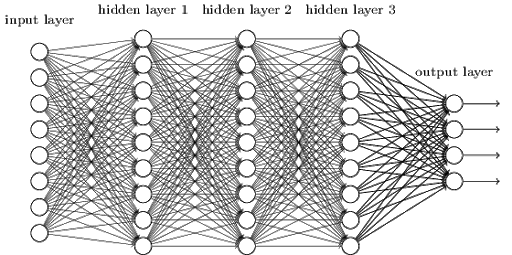
\includegraphics[scale=0.5]{fnn}
                \caption{A Feedforward Neural Network with 3 hidden layers(ref. Michael A. Nielsen, Neural Networks and Deep Learning, Determination Press', 2015)}
                \label{fig:fnn}
            \end{figure}
            This general but still basic form of Neural Network is known as \textit{Feed Forward Neural Network} Fig. \ref{fig:fnn}. 
        \subsection{Training}

            There are still a couple of important pieces left to define to develop a properly working Neural Network. For instance, how are parameters computed? And in particular, with respect to what we compute them? 
            \subsubsection{Loss Function}
                Before we realized that our goal is to maximize the approximation of the ground-truth input-output relation that lies under the data, therefore there is a need to
                introduce some metric to quantify this approximization. Call \textit{loss function} $ L(f_{\theta}\left(x\right), y) \colon \mathcal{Y} \times \mathcal{Y} \to \mathbb{R_+}$ 
                such metric. Common choices are (ref.):
                \begin{itemize}
                    \item Least Square: $\norm{f_{\theta}\left(x\right) - y}^2$ for regression tasks 
                    \item Binary Cross-Entropy: $y \log (f_{\theta}(x))+(1-y) \log (1-f_{\theta}(x))$ for binary classification  
                    \item Categorical Loss Function: $-\sum_{c=1}^{C} y_{c} \log \left(f_{\theta}(x)_c\right)$ for mulicategory classification with $C$ classes.
                \end{itemize}
                Intuitively, a good loss function will map bad approximations to high values and good approximations to smaller ones.
                Nevertheless, those are only point-wise estimates of the error, hence the best empirical solution learnable from the training set $ S $ would be 
                \begin{equation}
                    \label{erm}
                    \displaystyle{  \min_{\theta}  \frac{1}{n} \sum_{i=1}^{n} L\left(f_{\theta}\left(x_{i}\right), y_{i}\right) }
                \end{equation}
                which is called \textit{empirical risk minimization}.
            \subsubsection{Gradient Descent}
               So far we have described, given an input $ \mathbf{x} $, how we can compute the output of a feedforward neural network by means of compositions of dot products 
               and non-linear transformations between matrices, starting from the first to the very last of the layers in what is called a \textit{forward pass}. As it turns out, to attempt to solve \ref{erm} we need to follow the exact
               opposite path. Indeed, every optimization algorithm used in practice makes use of the same subroutine called Backpropagation (ref.  ) introduced in the 1970s, which allows to compute, starting from the output layer
               and going backwards, the partial derivative of the loss function with respect to each weight in the network. Moreover it does so efficiently requiring only one \textit{backward pass}.

               Let $i^l = W_l z_{l-1} + b_l$ be the weighted input to the $l$-th layer, then the key observation is that the only way $ W_l $ can affect the loss function is by affecting linearly
               the next layer which in turn affects its next layer and so on. In particular assume we add a little change $\Delta i_{j}^{l} $ to the $j$-th 
               element of $ i^l $ so that the neuron will output $ \sigma \left(i_{j}^{l} + \Delta i_{j}^{l}\right) $, this change will
               eventually propagates in the network causing the overall loss $LS$ to change by an amount $\frac{\partial LS}{\partial i_{j}^{l}} \Delta i_{j}^{l}$. For brevity,
               denote the gradient of the weighted input on the j-th neuron $ \delta^{l}_{j} = \frac{\partial LS}{\partial i^{l}_{j}} $, then the following holds:
               \begin{equation}
                 \delta^{L}_{j} = \frac{\partial LS}{\partial i^{L}_{j}} = \frac{\partial LS}{\partial z^{L}_{j}}\frac{\partial z^{L}_{j}}{\partial i^{L}_{j}} \\
                                =\frac{\partial LS}{\partial z^{L}_{j}} \sigma_{L}^{\prime}(i^{L}_{j})
               \end{equation}
               and equally, taking into account the whole output layer
               \begin{equation}
                    \label{bp1}
                    \delta^{L}=\nabla_{z^L} LS \odot \sigma^{\prime}(i^{L})
               \end{equation}
               where $ \odot $ is the element-wise product and $ \nabla_{x} $ the vector of the partial derivatives $ \partial LS / \partial x $. 
               That is, the gradient with respect to the weighted input to the last layer is given, using the chain rule, by the gradient with respect to the activation of the last layer times the derivative
               of the last activation function. Similarly, for any hidden layer $ l $ we note that:
               \begin{equation}
                \label{bp2}
                    \delta^{l}=\left((W^{l+1})^{T} \delta^{l+1}\right) \odot \sigma^{\prime}(i^{l})
                \end{equation}
                When we apply the transpose weight matrix, $(W^{l+1})^{T}$, think intuitively of this as moving the previous layer's gradient backward, giving a measure of the gradient at the output of the $l$-th layer. 
                We then take the product $\sigma^{\prime}(i^{l})$ which again moves the gradient backward through the activation function in layer $l$, giving the gradient of the weighted input to layer $l$.

                By combining \ref{bp1} with \ref{bp2} we can compute the gradient $\delta^{l}$ for any layer in the network. We start by using \ref{bp1} to compute on the last layer, 
                then apply equation \ref{bp2} to compute $\delta^{L-1}$, then the same equation again to compute $\delta^{L-2}$, and so forth, 
                all the way back until the input layer. Since our intent is to retrieve the gradients for every weights of the network, we are left to 
                show how $ \delta^l $ relates to them, here we provide such relation without giving an explicit proof which instead can be found in many
                texts like (ref Nielsen chapter 2).
                \begin{equation}
                    \frac{\partial LS}{\partial b^{l}_{j}} = \delta^{l}_{j}
                \end{equation}
                \begin{equation}
                    \frac{\partial LS}{\partial w^{l}_{i,j}} = z^{l-1}_i \delta^{l}_{j}.
                \end{equation}
                Remark how we already know how to compute each element on the right sides of these equations, moreover, given that the activation function
                and its derivative is efficiently computable, we will be able to efficiently get the seeked gradients in just one pass.
                It is worth mention that Backpropagation is actually a special case of a more generic set of programming techniques that go under
                the name of \textit{Automatic Differentiation} (Ref. ) to numerically evaluate the derivative of a function specified by a computer program.
                Such techniques are usually implemented in modern numerical libraries building variations of a data structure called \textit{computational graph}.
                Well known examples are \textit{Autograd} in \textit{Pytorch} (Ref. ) or \textit{GradientTape} in \textit{TensorFlow} (Ref. ).

               What does it mean to be able to compute partial derivatives of the loss? It means being able to understand where and how 
               the loss decreases and thus we can exploit such information to find better and better weights solutions. 
               This is the idea behind the Gradient Descent algorithm (Ref. ). In particular, the gradient of a weight is nothing but the
               direction inside the weight-space where the loss function is increasing, therefore what we want to do is to follow the opposite
               direction. Formally, this translates in the following weight update rules:
               \begin{equation}
                    w^{t}_{l} \rightarrow w_{l}^{t+1}=w^{t}_{l}-\frac{\eta}{n} \sum_{j} \frac{\partial LS_{\mathbf{x}_{j}}}{\partial w^{t}_{l}}
               \end{equation}
               \begin{equation}
                b^{t}_{l} \rightarrow b^{t+1}_{l}=b^{t}_{l}-\frac{\eta}{n} \sum_{j} \frac{\partial LS_{\mathbf{x}_{j}}}{\partial b^{t}_{l}}
               \end{equation}

            where $w_{l}^{t}$ are the values of the weights for layer $l$-th during the $t$-th pass, $\eta$ is a small positive constant called \textit{learning rate}
            chosen by the user accordingly and the gradients are averaged among all samples in the training set. 
            \begin{figure}[h!]
                \centering
                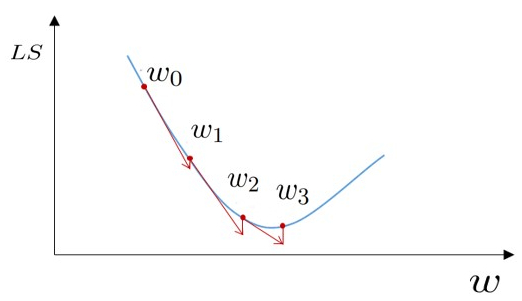
\includegraphics[scale=0.5]{gd}
                \caption{A 1-D representation of 4 gradient descent steps}
                \label{fig:gd}
            \end{figure}
            Most importantly, note how we take the negative of the gradients, meaning that we are following the direction in which the loss decreases \ref{fig:gd}. The distance
            between two consecutives weights $\Delta_{w^t}$ well be directly proportional to both the learning rate picked and the averaged gradient.

            In practice, however, when very often we are deling with thousands or milions of data points, becomes unfeasable to compute every pass over
            the entire training set, thus what is done is to split the data into so called \textit{mini-batches} and then apply the
            update rules on each mini-batch until we scanned the whole data. The entire scan is called \textit{epoch} and the 
            resulting algorithm Stochastic Gradient Descent (Ref. ). Lastly, the size of a mini-batch is another hyperparameter 
            that should be tuned by the developer, keeping in mind that the bigger the size the more stable will be our training
            the smaller the size the faster the training.


        \subsection{Activation Functions}
        \subsection{CNNs: Convolutional Neural Networks}

        \subsection{From Neural Networks to Deep Neural Networks}
        

    \section{Adversarial Examples Theory}

        Formal definition of what is an adversarial attacks plus currently well known attacks

    \section{Defenses}

        Review of the literature on defenses to improve robustness: provable robustness, adversarial training

    \section{Kernel Based Activation Functions}


\chapter{Related Works}

    \section{K-Winners Take All}
    \section{Smooth Adversarial Training}


\chapter{Solution Approach}
 
    Comparing the activations's distributions for different activation functions (ReLU, KWTA, Kafs) 
    seem to suggest Kafs might be good candidates to improve model robustness 

    \section{Lipschitz Constant Approach}

        On the limitations of current Lipischitz-Constant based approaches especially when involving Kafs

    \section{Fast is Better than Free Adversarial Training}

        Adversarial training (Madry et al.) and current methods to improve the efficiency (Fast is better than free)


\chapter{Evaluation}

    \section{VGG Inspired Architectures Results}

    \section{Explofing Gradients with KafNets}

        The exploding gradients problem with KafResNet, why is it happening? (still to clarify)

    \section{ResNet20 Inspired Architectures Results}


\chapter{Future Works}

    Different Kernels, resolve the exploding gradient problem and scale to ImageNet
    Perform more adaptive attacks to assess the robustness of kafresnets as is the current standard (Carlini et al.)


\chapter{Conclusions}

    This thesis tries to add to the bag of evidences in literature that smoother architectures might benefit improvements in adversarial resiliency
    
    
\appendix


\backmatter
% bibliography
%\cleardoublepage
%\phantomsection
%\bibliographystyle{sapthesis} % BibTeX style
%\bibliography{bibliography} % BibTeX database without .bib extension

\end{document}
